\chapter{Event Categorisation}
\label{chap:event_select}

\newpage
\section{Introduction}
Once a set of candidate photons is assembled we tag and categorise events using extra final-state objects which are characteristic of particular Higgs production modes.
The objective of this tagging procedure is to enhance signficance and to construct categories of events with superior mass resolution.


\section{The Diphoton BDT}


\section{Top Fusion Tag}

\subsection{Leptonic}
\subsection{Hadronic}


\section{Associated Production Tag}

\subsection{Leptonic}
\subsection{Hadronic}
\subsection{MET}


\section{Vector Boson Fusion Tag}

\subsection{Introduction}

\subsection{Legacy Tag}


\subsection{Jet Images}
The spatial distribution and properties of a jet's constituent particles encodes information about the jet's originating parton. 

\begin{figure}[h!]

    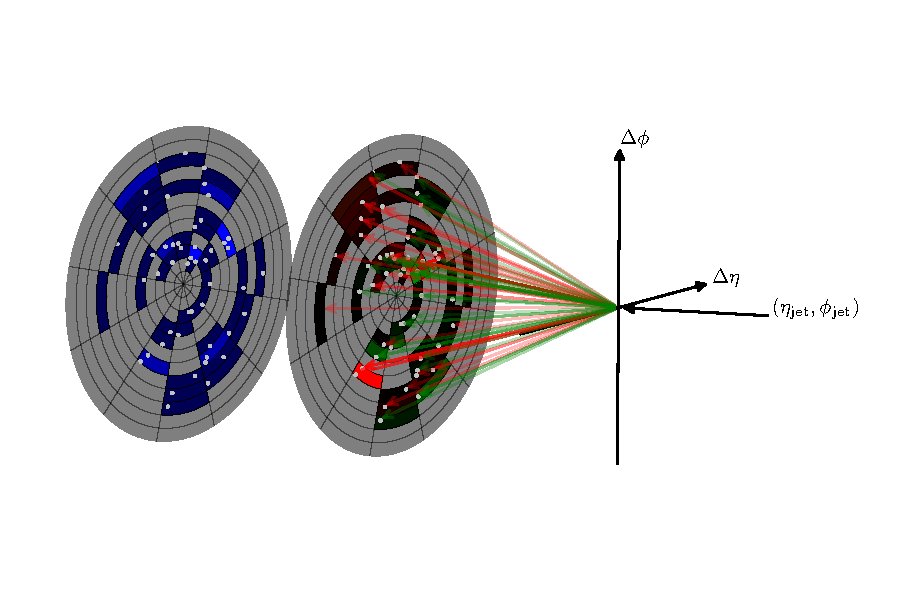
\includegraphics[width=\textwidth]{figures/event_selection/jet_diagram_RGB.pdf}
    \begin{center}
        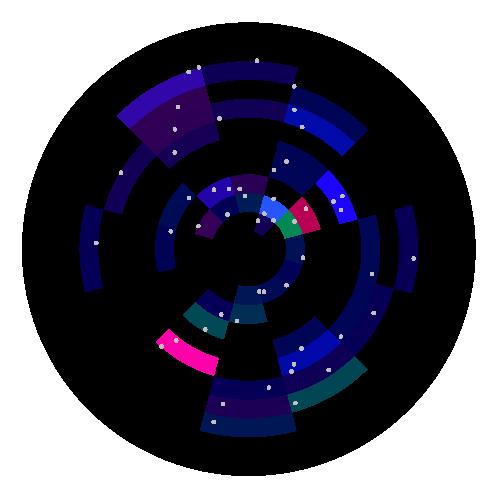
\includegraphics[width=0.49\textwidth]{figures/event_selection/full_image_polar.pdf}
        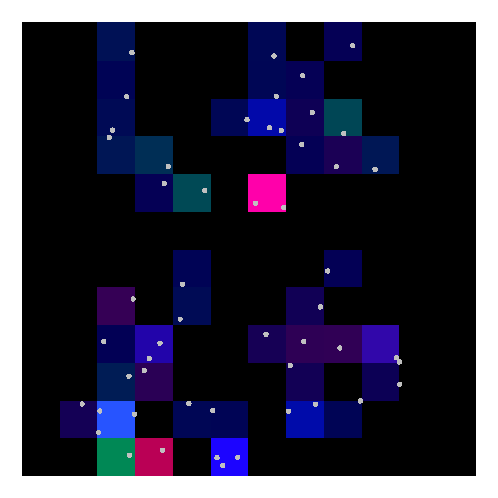
\includegraphics[width=0.49\textwidth]{figures/event_selection/full_image_rect.pdf}
    \end{center}

    \caption{\textbf{Top:} 
             construction of single-jet image from jet constituents. Arrows correspond to individial PF candidates where red arrows are charged, green are neutral and the opacity corresponds to $p_{T}$.
             The red channel measures charged candidate $p_T$ deposition in each pixel, 
             the green channel is neutral charged candidates $p_T$ deposition, 
             and the blue channel is the number of candidates in each pixel (multiplicity). 
             Multiplicity channel is drawn separately so the charged and neutral channels can be seen clearly. Black pixels are lightened to show coloured pixels more clearly.\\
             \textbf{Bottom:} 
             the final image with all the channels together.}
    \label{fig:event_categorisation:jet_image}

\end{figure}


\subsection{New Tag}
The objective of the new tag is to use jet images and a dense CNN to enhance VBF signal extraction, especially VBF vs Gluon Fusion discrimination. 

\subsection{Design}
\subsection{Model Optimisation}
\subsection{Final Model}
\subsection{Model Performance}
\subsection{Interpretation}

\section{Untagged}
